\documentclass[12pt, a4paper]{article}%{{{
\usepackage[utf8]{inputenc}
\usepackage[T1]{fontenc}
\usepackage[a4paper,left=2cm,right=2cm,top=2cm,bottom=2cm]{geometry}
\usepackage[frenchb]{babel}
\usepackage{libertine}
\usepackage{float}
\usepackage{hyperref}
\usepackage{amsfonts}
\usepackage{amssymb}
\usepackage[dvipsnames]{xcolor}
\usepackage[pdftex]{graphicx}

\setlength{\parindent}{0cm}
\setlength{\parskip}{1ex plus 0.5ex minus 0.2ex}
\newcommand{\hsp}{\hspace{20pt}}
\newcommand{\HRule}{\rule{\linewidth}{0.5mm}}

\begin{document}

\begin{titlepage}
  \begin{sffamily}
  \begin{center}

    % Upper part of the page. The '~' is needed because \\
    % only works if a paragraph has started.
    
\includegraphics[scale=1]{Images/polytechnique_genie_gauche_fr_rgb.png}~\\[1.5cm]

    \textsc{\LARGE École Polytechnique Montréal}\\[2cm]

    \textsc{\Large INF8405 : Informatique Mobile}\\[1.5cm]

    % Title
    \HRule \\[0.4cm]
    { \huge \bfseries TP2 : Intégration de Maps\\[0.4cm] }

    \HRule \\[2cm]
    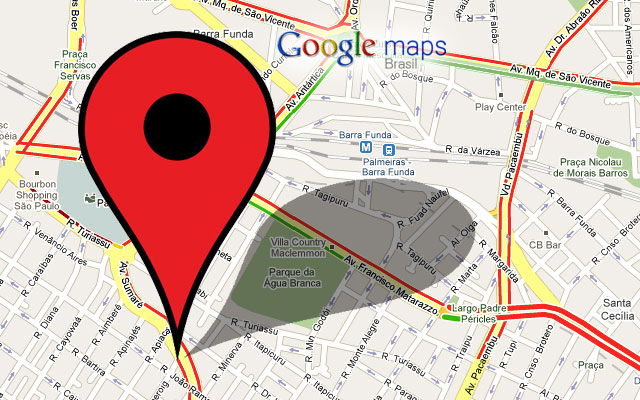
\includegraphics[scale=0.3]{Images/Google-Maps.jpg}\\[2cm]

    % Author and supervisor
    \begin{minipage}{0.4\textwidth}
      \begin{flushleft} \large
          Philippe TROCLET \textsc{1815208}\\
          Alexandre  MAO \textsc{1813566}\\
          Fabien  BERQUEZ \textsc{1800325}\\
      \end{flushleft}
    \end{minipage}
    \begin{minipage}{0.4\textwidth}
      \begin{flushright} \large
        \emph{Soumis à :} M. Aurel Josas RANDOLF\\
        \emph{Soumis le :} 23 Mars 2016  \\
        \emph{Session} Hiver 2016 
      \end{flushright}
    \end{minipage}

    \vfill

  \end{center}
  \end{sffamily}
\end{titlepage}%}}}


\section{Introduction}
L'objectif du TP n°2 était de développer une application destinée à faciliter les rencontres entre membres d'un groupe. Plus précisément, les requis de l'application étaient centrés autour de l'utilisation de différentes ressources, comme le GPS, le calendrier des membres, des API externes comme Google Maps ou Google Places. L'application devait permettre à chaque personne du groupe de définir son profil (nom, courriel, lieux de rencontre préférés) et s'il était organisateur ou non. Une fois ceci fait, et le groupe constitué, l'application, en se basant sur les lieux de rencontre préférés et la position géographique des membres du groupe, proposait trois options de rendez-vous. Les membres du groupe devaient alors choisir chacun l'option qui leur convenait le mieux. Le résultat était transmis à l'organisateur qui pouvait alors définir un lieu et une heure, d'après les disponibilités des membres du groupes, ainsi qu'un petit texte présentant le choix qu'il a retenu. Les informations étaient alors transmises à tous les membres du groupe afin que ceux-ci disposent des informations nécessaires pour aller au rendez-vous.\\
D'un point de vue technique, l'application a pour requis d'être exécutable sur les plateformes Android supportant l'API 18 et supérieures (jusqu'à la version 23 pour la plus récente), c'est à dire des versions d'Android 4.3 à Android 6.0. L'application doit être capable d'être utilisable, avec des fonctionnalités réduites, même lorsque la connexion au réseau cellulaire ou Wi-Fi n'est pas possible, ce qui a eu un impact sur les choix d'implémentation réalisés lors du développement de cette application.  


\section{Présentation générale}

\section{Présentation Technique}
    \subsection{Partie Serveur}
    Les différents utilisateurs doivent communiquer entre eux afin de pouvoir voter, mais aussi pour connaître la position de chacun
des utilisateurs. Une telle communication nécessite la présence d'un serveur connu de tous. Pour mettre en place une serveur nous
avons choisi d'utiliser le service cloud \textit{firebase}. Les données sont stockées sous le format jason sur le serveur. On peut
alors les récupérer via leur id (générés par l'API firebase).
\newline

Cette solution a plusieurs avantages:
\begin{enumerate}
    \item la présence d'une API déjà testée et éprouvée, ce qui limite le nombre de bugs. Et permet de ne pas réinventer la roue.
    \item la présence de mécanismes de pour écouter des données sur le serveur et être informé en cas de modification.
    \item une grande communauté d'utilisateurs, ce qui facilite la recherche d'information en cas de débogguage.
\end{enumerate}

Ainsi, les coordonnées (longitude/latitude) de chaque utilisateur peuvent être mises à jour sur le serveur en temps réel (ou
presque). Il suffit pour cela d'envoyer ces nouvelles coordonnées sur le serveur à chaque fois que la \textit{callback} associée
au changement de position dans \textit{maps} est appelée. (L'envoie se ferait dans la dite \textit{callback}). Les autres membres
du groupe n'aurait qu'à écouter ces coordonnées sur le serveur afin d'être informé de tous changements de position.
\newline

Cette approche est un peu gourmande en terme de réseau, aussi il est possible de mettre à jour les données que à des moments jugés
opportuns. On obtient alors une meilleure utilisation du réseau mais on perd le temps réel.

\section{Critiques et suggestions}
\end{document}
